\documentclass[journal, a4paper]{IEEEtran}

% some very useful LaTeX packages include:
\usepackage{siunitx}
\usepackage{cite}      % Written by Donald Arseneau
                        % V1.6 and later of IEEEtran pre-defines the format
                        % of the cite.sty package \cite{} output to follow
                        % that of IEEE. Loading the cite package will
                        % result in citation numbers being automatically
                        % sorted and properly "ranged". i.e.,
                        % [1], [9], [2], [7], [5], [6]
                        % (without using cite.sty)
                        % will become:
                        % [1], [2], [5]--[7], [9] (using cite.sty)
                        % cite.sty's \cite will automatically add leading
                        % space, if needed. Use cite.sty's noadjust option
                        % (cite.sty V3.8 and later) if you want to turn this
                        % off. cite.sty is already installed on most LaTeX
                        % systems. The latest version can be obtained at:
                        % http://www.ctan.org/tex-archive/macros/latex/contrib/supported/cite/

\usepackage{graphicx}   % Written by David Carlisle and Sebastian Rahtz
                        % Required if you want graphics, photos, etc.
                        % graphicx.sty is already installed on most LaTeX
                        % systems. The latest version and documentation can
                        % be obtained at:
                        % http://www.ctan.org/tex-archive/macros/latex/required/graphics/
                        % Another good source of documentation is "Using
                        % Imported Graphics in LaTeX2e" by Keith Reckdahl
                        % which can be found as esplatex.ps and epslatex.pdf
                        % at: http://www.ctan.org/tex-archive/info/

%\usepackage{psfrag}    % Written by Craig Barratt, Michael C. Grant,
                        % and David Carlisle
                        % This package allows you to substitute LaTeX
                        % commands for text in imported EPS graphic files.
                        % In this way, LaTeX symbols can be placed into
                        % graphics that have been generated by other
                        % applications. You must use latex->dvips->ps2pdf
                        % workflow (not direct pdf output from pdflatex) if
                        % you wish to use this capability because it works
                        % via some PostScript tricks. Alternatively, the
                        % graphics could be processed as separate files via
                        % psfrag and dvips, then converted to PDF for
                        % inclusion in the main file which uses pdflatex.
                        % Docs are in "The PSfrag System" by Michael C. Grant
                        % and David Carlisle. There is also some information
                        % about using psfrag in "Using Imported Graphics in
                        % LaTeX2e" by Keith Reckdahl which documents the
                        % graphicx package (see above). The psfrag package
                        % and documentation can be obtained at:
                        % http://www.ctan.org/tex-archive/macros/latex/contrib/supported/psfrag/

\usepackage{subfigure} % Written by Steven Douglas Cochran
                        % This package makes it easy to put subfigures
                        % in your figures. i.e., "figure 1a and 1b"
                        % Docs are in "Using Imported Graphics in LaTeX2e"
                        % by Keith Reckdahl which also documents the graphicx
                        % package (see above). subfigure.sty is already
                        % installed on most LaTeX systems. The latest version
                        % and documentation can be obtained at:
                        % http://www.ctan.org/tex-archive/macros/latex/contrib/supported/subfigure/

\usepackage{url}        % Written by Donald Arseneau
                        % Provides better support for handling and breaking
                        % URLs. url.sty is already installed on most LaTeX
                        % systems. The latest version can be obtained at:
                        % http://www.ctan.org/tex-archive/macros/latex/contrib/other/misc/
                        % Read the url.sty source comments for usage information.

%\usepackage{stfloats}  % Written by Sigitas Tolusis
                        % Gives LaTeX2e the ability to do double column
                        % floats at the bottom of the page as well as the top.
                        % (e.g., "\begin{figure*}[!b]" is not normally
                        % possible in LaTeX2e). This is an invasive package
                        % which rewrites many portions of the LaTeX2e output
                        % routines. It may not work with other packages that
                        % modify the LaTeX2e output routine and/or with other
                        % versions of LaTeX. The latest version and
                        % documentation can be obtained at:
                        % http://www.ctan.org/tex-archive/macros/latex/contrib/supported/sttools/
                        % Documentation is contained in the stfloats.sty
                        % comments as well as in the presfull.pdf file.
                        % Do not use the stfloats baselinefloat ability as
                        % IEEE does not allow \baselineskip to stretch.
                        % Authors submitting work to the IEEE should note
                        % that IEEE rarely uses double column equations and
                        % that authors should try to avoid such use.
                        % Do not be tempted to use the cuted.sty or
                        % midfloat.sty package (by the same author) as IEEE
                        % does not format its papers in such ways.

\usepackage{amsmath}    % From the American Mathematical Society
                        % A popular package that provides many helpful commands
                        % for dealing with mathematics. Note that the AMSmath
                        % package sets \interdisplaylinepenalty to 10000 thus
                        % preventing page breaks from occurring within multiline
                        % equations. Use:
%\interdisplaylinepenalty=2500
                        % after loading amsmath to restore such page breaks
                        % as IEEEtran.cls normally does. amsmath.sty is already
                        % installed on most LaTeX systems. The latest version
                        % and documentation can be obtained at:
                        % http://www.ctan.org/tex-archive/macros/latex/required/amslatex/math/



% Other popular packages for formatting tables and equations include:

\usepackage{array}
% Frank Mittelbach's and David Carlisle's array.sty which improves the
% LaTeX2e array and tabular environments to provide better appearances and
% additional user controls. array.sty is already installed on most systems.
% The latest version and documentation can be obtained at:
% http://www.ctan.org/tex-archive/macros/latex/required/tools/

% V1.6 of IEEEtran contains the IEEEeqnarray family of commands that can
% be used to generate multiline equations as well as matrices, tables, etc.

% Also of notable interest:
% Scott Pakin's eqparbox package for creating (automatically sized) equal
% width boxes. Available:
% http://www.ctan.org/tex-archive/macros/latex/contrib/supported/eqparbox/

% *** Do not adjust lengths that control margins, column widths, etc. ***
% *** Do not use packages that alter fonts (such as pslatex).         ***
% There should be no need to do such things with IEEEtran.cls V1.6 and later.


% Your document starts here!
\begin{document}
% Define document title and author
	\title{ BH++: A Black Hole Geodesics Integrator in C++}
	\author{Arnau Quera-Bofarull}	
	\markboth{Numerical Methods}{A. Quera-Bofarull}
	\maketitle

% Write abstract here
\begin{abstract}
	The short abstract (50-80 words) is intended to give the reader an overview of the work.
\end{abstract}

% Each section begins with a \section{title} command
\section{Introduction}
	% \PARstart{}{} creates a tall first letter for this first paragraph
	\IEEEPARstart{G}{eneral} 

% Main Part
\section{The integrator algorithm}

\section{Testing the algorithm}
In this section, we initialize our solver with initial conditions for known sceneraios: the existence of a circular orbit for photons at $R=\frac{3}{2}R_s$, and the planetary system formed by the Sun, the Earth and Jupiter (ignoring the effects of the planets to the metric).
\subsection{Photon geodesics}
The effective potential for massless particles is
\begin{equation}
	V(R) = \frac{L^2}{2R^2} - \frac{GML^2}{c^2R^3},
\end{equation}
which has an extremum at
\begin{equation}
	\frac{dV}{dR} = 0 \; ; \; R = \frac{3GM}{c^2} = \frac{3}{2} R_s,
\end{equation}
independently of its angular momentum. This corresponds to the circular photon orbit, which is unstable as we can clearly see from the shape of the effective potential in figure \ref{fig::veffphotons}.
\begin{figure}[!hbt]
	\begin{center}
	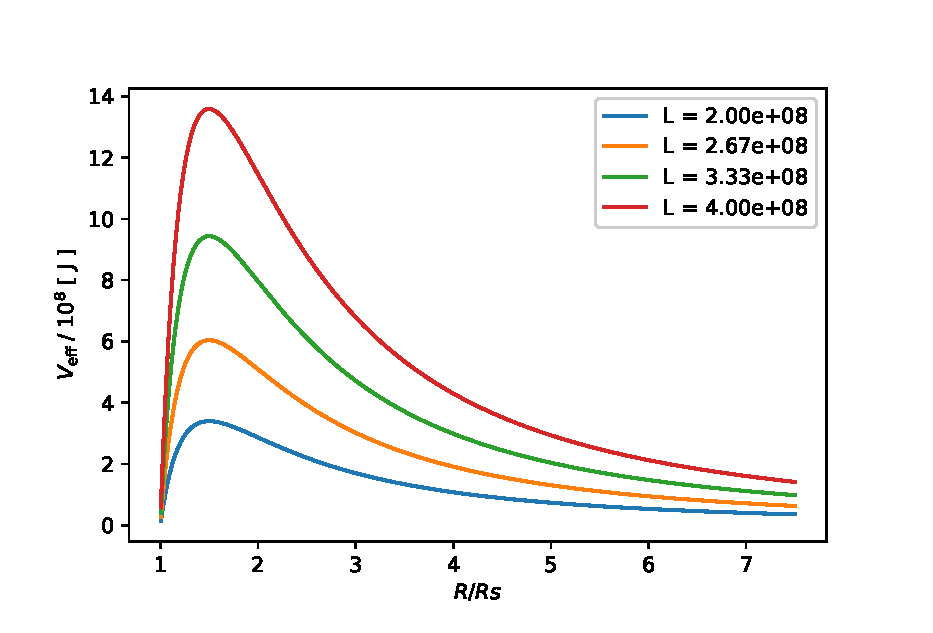
\includegraphics[width=\columnwidth]{Veff_photon.eps}
	\caption{Effective potential for a photon close to the black hole.}
	\label{fig::veffphotons}
\end{center}
\end{figure}

We initialize a set of 15 photons, one of them at the expected circular orbit, with an arbitrarily chosen specific angular momentum $L=10^8$ $\si[per-mode=symbol]{\meter^2\per \second}$. The results are shown in figure \ref{fig::photon_geodesics}. As we can see, the photon with $R0=1.5R_s$ traces a circular orbit as expected, while the outer photons escape from the black hole and the inner ones get trapped. This is consistent with the extremum being a maximum, hence the circular orbit is unstable. Our integrator gives the same result even after thousands of revolutions, confirming its numerical stability. 
\begin{figure}[!hbt]
	\begin{center}
	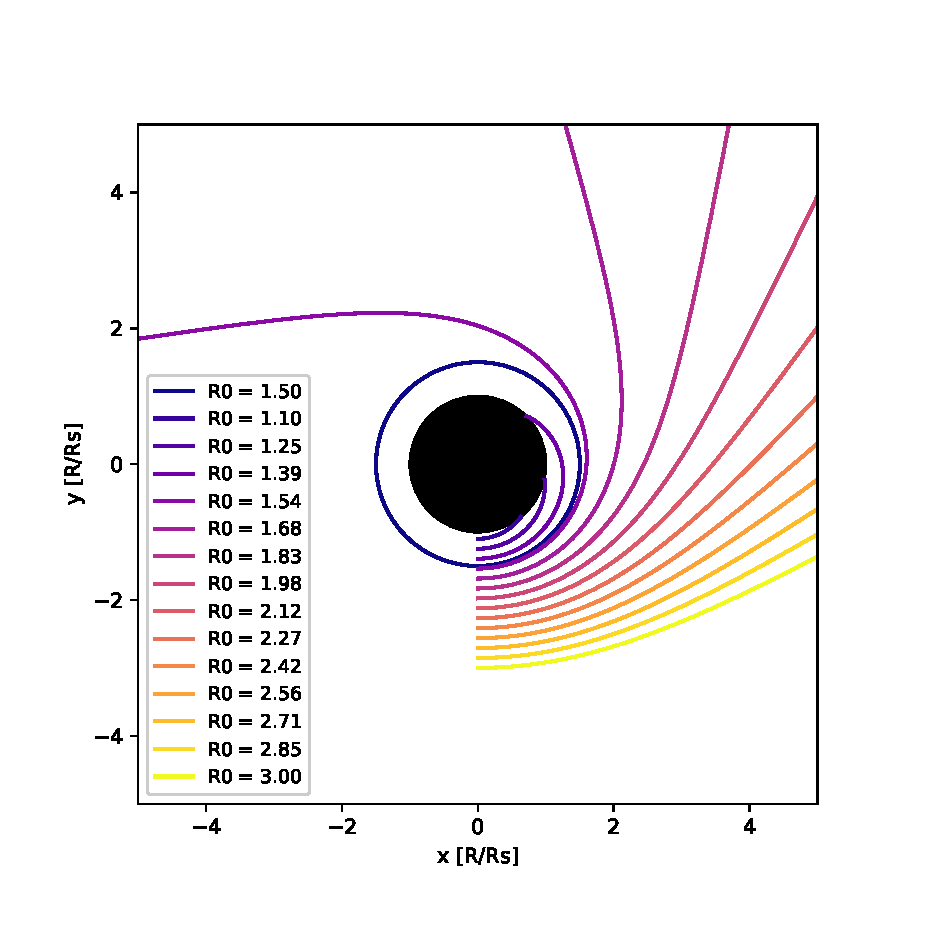
\includegraphics[width=\columnwidth]{photon_geodesics.eps}
	\caption{Set of 15 photon orbits initialized at different radii. $R0=1.5$ confirms the photon circular orbit.}
	\label{fig::photon_geodesics}
\end{center}
\end{figure}

\subsection{Massive particle geodesics}
From [REF] the effective potential for massive particles is
\begin{equation}
	V(R) = \frac{c^2}{2} - \frac{GM}{R} + \frac{L^2}{2R^2} - \frac{GML^2}{c^2R^3},
\end{equation}
which differs from the Newtonian one by the last factor $\sim r^{-3}$ and the rest energy of the particle. We find the circular orbits at the extrema of the effective potential,
\begin{equation}
	\frac{dV}{dr} = 0,
\end{equation}
\begin{equation}
	R_{\pm} = \frac{L^2 \pm \sqrt{ L^4 - \frac{12 G^2 M^2 L^2}{ c^2} } }{2 G M},
\end{equation}
that now depend on angular momenta as opposed to the massless case. The shape of the effective potential for different $L$ is plotted in figure \ref{fig::Veff_massive}
\begin{figure}[!hbt]
	\begin{center}
	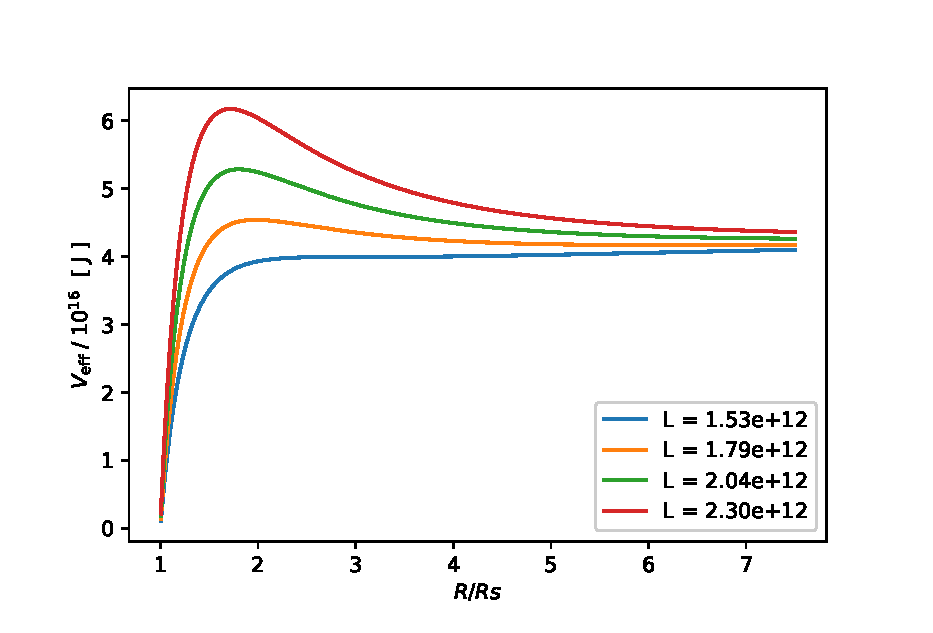
\includegraphics[width=\columnwidth]{Veff_massive.eps}
	\caption{Effective potential of massive particles for different values of the angular momentum.}
	\label{fig::Veff_massive}
\end{center}
\end{figure}
We initialize 6 massive particles with different angular momentum at the extrema position. We see that they indeed form circular orbits in figure \ref{fig::massive_geodesics}.
\begin{figure}[!hbt]
	\begin{center}
	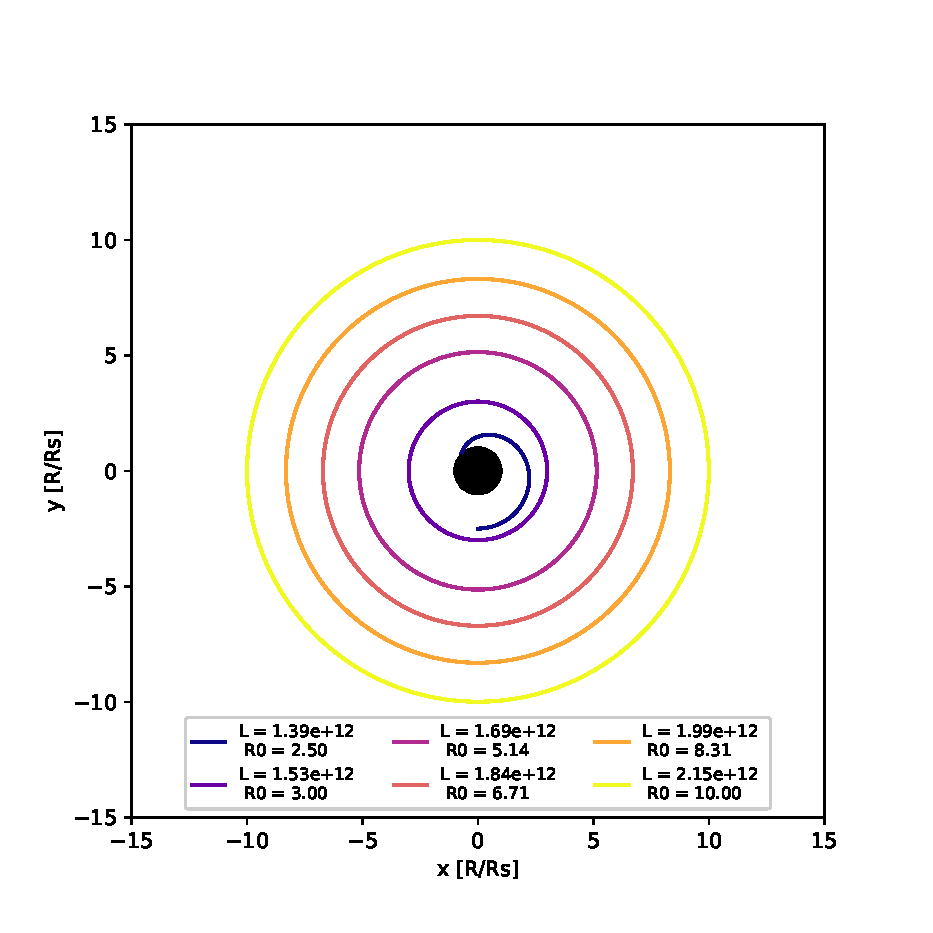
\includegraphics[width=\columnwidth]{massive_geodesics.eps}
	\caption{Set of 6 massive particle orbits initialized at different radii and angular momenta. $R_0=3$ confirms the innermost circular orbit.}
	\label{fig::massive_geodesics}
\end{center}
\end{figure}

There is a characteristic radius below which no circular orbits exist, 
\begin{equation}
	L^4 < \frac{ 12 G^2 M^2 L^2}{ c^2} \rightarrow L < \sqrt{12 } G M,
\end{equation}
which corresponds to $r<3 R_s$. No particle can orbit in a circular fashion inside this radius, in contrast to the Newtonian case.

\subsection{Newtonian limit: The Solar System}
The last check we perform is initializing the solver with a planteray system consisting of the Earth, Jupiter and the Sun as seen in figure \ref{fig::solarsystem}. The eccentricity of the orbits is $\varepsilon = 0.0034$ for the Earth and $\varepsilon=0.123$ for Jupiter. The disagreement on Jupiter's eccentricity (compared to the observed one) is due to ignoring the gravitational fields from other planets. 
\begin{figure}[!hbt]
	\begin{center}
	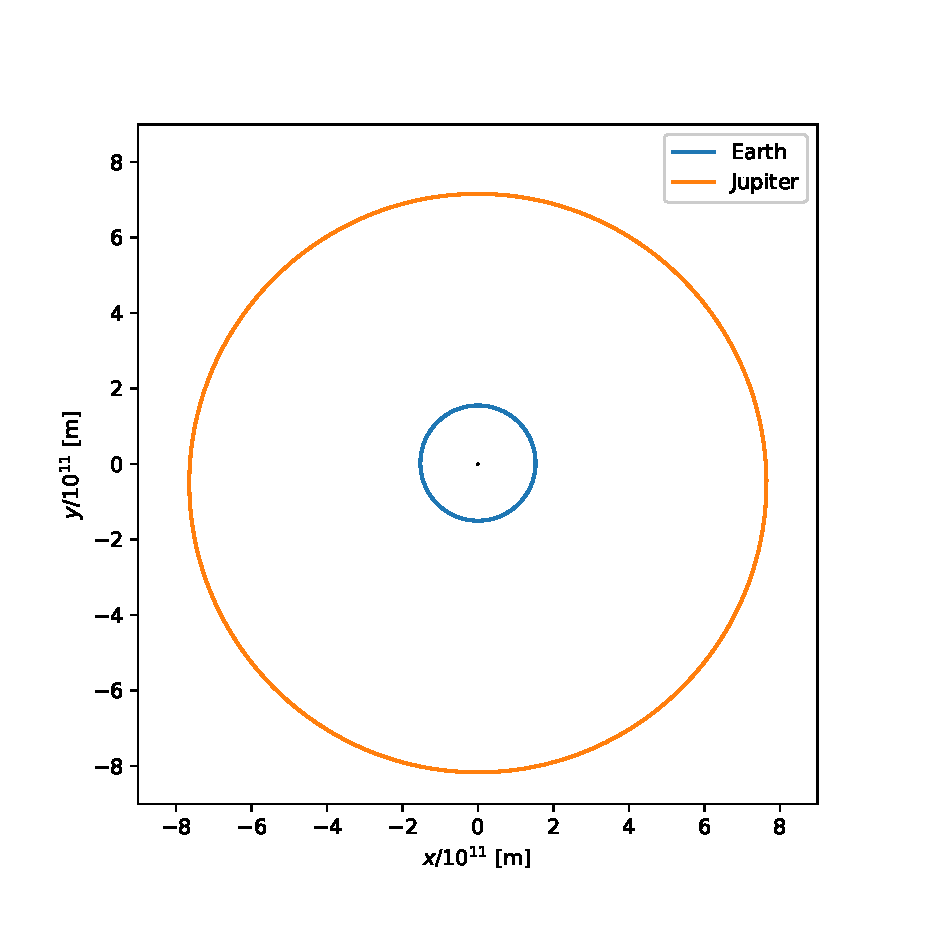
\includegraphics[width=\columnwidth]{SolarSystem.eps}
	\caption{Orbits of the Earth and Jupiter around the sun.}
	\label{fig::solarsystem}
\end{center}
\end{figure}
\section{Conclusion}
	This section summarizes the paper.

% Now we need a bibliography:
\begin{thebibliography}{5}

	%Each item starts with a \bibitem{reference} command and the details thereafter.
	\bibitem{HOP96} % Transaction paper
	J.~Hagenauer, E.~Offer, and L.~Papke. Iterative decoding of binary block
	and convolutional codes. {\em IEEE Trans. Inform. Theory},
	vol.~42, no.~2, pp.~429–-445, Mar. 1996.

	\bibitem{MJH06} % Conference paper
	T.~Mayer, H.~Jenkac, and J.~Hagenauer. Turbo base-station cooperation for intercell interference cancellation. {\em IEEE Int. Conf. Commun. (ICC)}, Istanbul, Turkey, pp.~356--361, June 2006.

	\bibitem{Proakis} % Book
	J.~G.~Proakis. {\em Digital Communications}. McGraw-Hill Book Co.,
	New York, USA, 3rd edition, 1995.

	\bibitem{talk} % Web document
	F.~R.~Kschischang. Giving a talk: Guidelines for the Preparation and Presentation of Technical Seminars.
	\url{http://www.comm.toronto.edu/frank/guide/guide.pdf}.

	\bibitem{5}
	IEEE Transactions \LaTeX and Microsoft Word Style Files.
	\url{http://www.ieee.org/web/publications/authors/transjnl/index.html}

\end{thebibliography}

% Your document ends here!
\end{document}
